\documentclass{article}
\usepackage{bm}
\usepackage{amsmath}
\usepackage{amssymb}
\usepackage{graphicx}
\usepackage[colorlinks=true,urlcolor=blue]{hyperref}
\usepackage{geometry}
\geometry{margin=1in}
\usepackage{multicol}
\usepackage{paralist}
\usepackage{todonotes}
\setlength{\marginparwidth}{2.15cm}
\usepackage{booktabs}
\usepackage{enumitem}
\graphicspath{{../}}
\usepackage{setspace}
\doublespacing

\newcommand{\norm}[1]{\left\lVert#1\right\rVert}
\newcommand\numberthis{\addtocounter{equation}{1}\tag{\theequation}}

\begin{document}

\section*{}
\begin{center}
  \centerline{\textsc{\LARGE Homework 3}}
  \vspace{0.5em}
  \centerline{\textsc{Regression, Gaussian Processes, and Boosting}}
  \vspace{1em}
  \textsc{\large Dana Van Aken} \\
\end{center}

\section*{Problem 1: Gaussian Processes}

\begin{enumerate}[label=(\alph*)]
\setlength\itemsep{1em}

\item A comparison of covariance functions: see figures~\ref{fig:1a1},~\ref{fig:1a2}, and~\ref{fig:1a3}.
\begin{figure}[H]
\centering
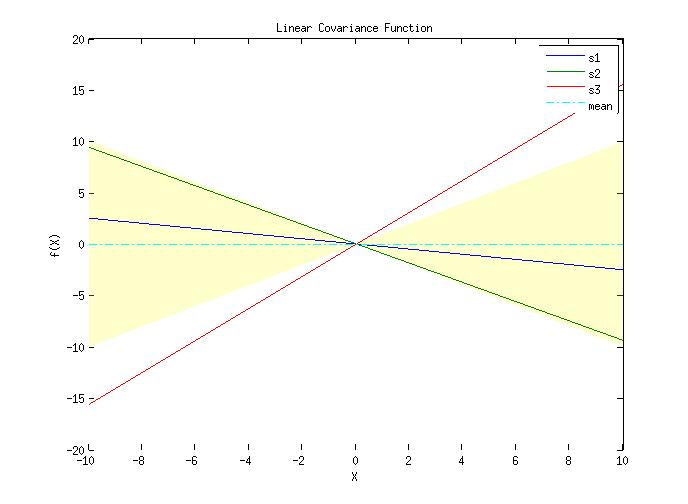
\includegraphics[width=0.8\textwidth]{1_a_1.jpg}
\caption{Linear Covariance Function}
\label{fig:1a1}
\end{figure}
\begin{figure}[H]
\centering
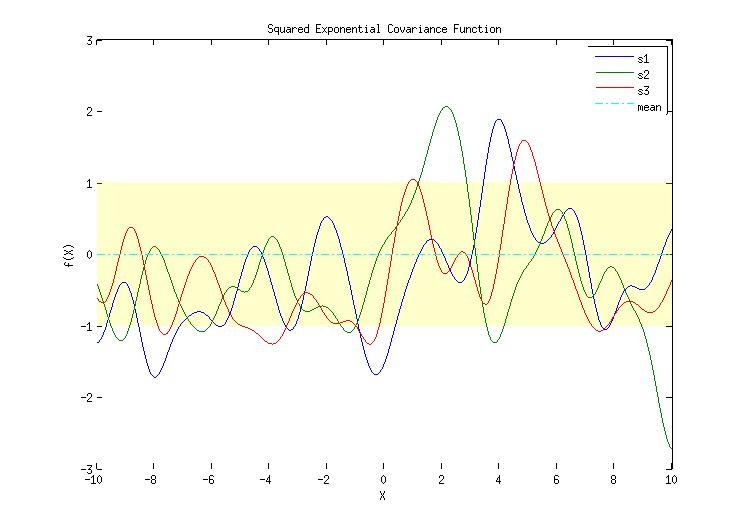
\includegraphics[width=0.8\textwidth]{1_a_2.jpg}
\caption{Square Exponential Covariance Function}
\label{fig:1a2}
\end{figure}
\begin{figure}[H]
\centering
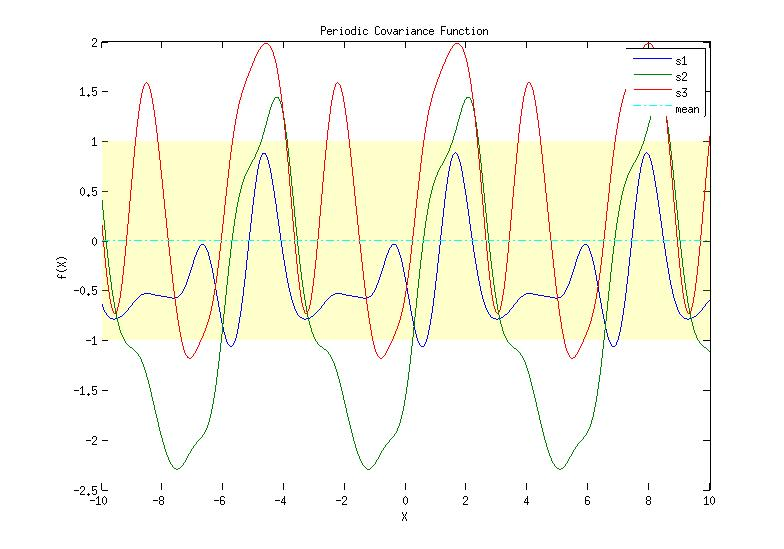
\includegraphics[width=0.8\textwidth]{1_a_3.jpg}
\caption{Periodic Covariance Function}
\label{fig:1a3}
\end{figure}

\item $\sigma^2$ affects the ``noisyness" of the output points, $y_i$.
Figure~\ref{fig:1b} shows that as we increase $\sigma^2$, the amount of noise (or "spikyness" in the graph) increases.

\begin{figure}[H]
\centering
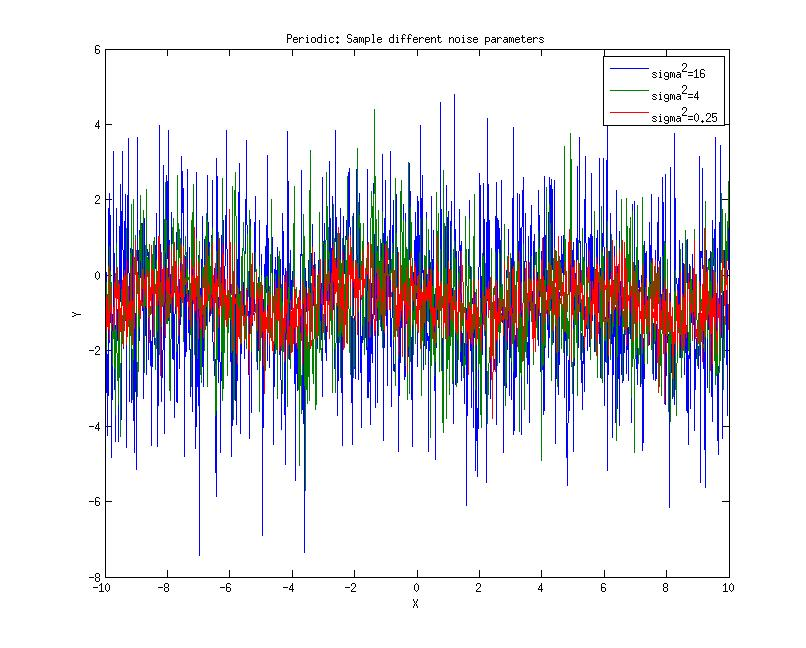
\includegraphics[width=0.8\textwidth]{1_b.jpg}
\caption{Sampling Different Gaussian Noise Parameters Using a Periodic Covariance Function}
\label{fig:1b}
\end{figure}

\item Show $p(x_1|x_2)\propto{}p(x_1,x_2)$ \\
We want to find $\mu_{x_1|x_2}$ and $\Sigma_{x_1|x_2}$ in:
\begin{align*}
p(x_1|x_2)&=Z\exp\Big(-\frac{1}{2}(x-\mu_{x_1|x_2})^T\Sigma_{x_1|x_2}^{-1}(x-\mu_{x_1|x_2}))\Big) \\
&=Z\exp\Big(-\frac{1}{2}(x^T\Sigma_{x_1|x_2}^{-1}x-x^T\Sigma_{x_1|x_2}^{-1}\mu_{x_1|x_2}
-\mu_{x_1|x_2}^T\Sigma_{x_1|x_2}^{-1}x+\mu_{x_1|x_2}^T\Sigma_{x_1|x_2}^{-1}\mu_{x_1|x_2})\Big) \\
&=Z\exp\Big(-\frac{1}{2}x^T\Sigma_{x_1|x_2}^{-1}x+x^T\Sigma_{x_1|x_2}^{-1}\mu_{x_1|x_2}
-\frac{1}{2}\mu_{x_1|x_2}^T\Sigma_{x_1|x_2}^{-1}\mu_{x_1|x_2})\Big) \numberthis \label{e1}
\end{align*}
where $Z=\frac{1}{\sqrt{(2\pi)^k|\Sigma_{x_1|x_2}|}}$
\[
\begin{bmatrix}
  x_1 \\ x_2
\end{bmatrix}
\sim{}N \Bigg(
\begin{bmatrix}
  \mu_1 \\ \mu_2
\end{bmatrix}
\begin{bmatrix}
  \Sigma_{11} & \Sigma{12} \\ \Sigma{21} & \Sigma{22}
\end{bmatrix}
\Bigg)
\]
Let $\Sigma^{-1}=\Lambda^{-1}$ such that
\[
\Sigma^{-1}=
\begin{bmatrix}
  \Sigma_{11} & \Sigma_{12} \\ \Sigma_{21} & \Sigma_{22}
\end{bmatrix}
^{-1}=
\begin{bmatrix}
  \Lambda_{11} & \Lambda_{12} \\ \Lambda_{21} & \Lambda_{22}
\end{bmatrix}
=\Lambda
\]
We can focus on the exponent since we want to find $\mu_{x_1|x_2}$ and $\Sigma_{x_1|x_2}$.
%\begin{equation}
%\begin{align*}
%-\frac{1}{2}(x-\mu)^T\Sigma^{-1}(x-\mu) 
%&=-\frac{1}{2}(x-\mu)^T\Sigma^{-1}(x-\mu) 
%\end{align*}
%\end{equation}
\begin{align*}
exp&=-\frac{1}{2}(x-\mu)^T\Sigma^{-1}(x-\mu) \\
&=-\frac{1}{2}
\begin{bmatrix}
  x_1 - \mu_1 \\ x_2 - \mu_2
\end{bmatrix}
^T
\begin{bmatrix}
  \Sigma_{11} & \Sigma_{12} \\ \Sigma_{21} & \Sigma_{22}
\end{bmatrix}
^{-1}
\begin{bmatrix}
  x_1 - \mu_1 \\ x_2 - \mu_2
\end{bmatrix} \\
&=-\frac{1}{2}
\begin{bmatrix}
  x_1 - \mu_1 \\ x_2 - \mu_2
\end{bmatrix}
^T
\begin{bmatrix}
  \Lambda_{11} & \Lambda_{12} \\ \Lambda_{21} & \Lambda_{22}
\end{bmatrix}
\begin{bmatrix}
  x_1 - \mu_1 \\ x_2 - \mu_2
\end{bmatrix}
\end{align*}
\begin{multline*}
=-\frac{1}{2}(x_1-\mu_1)^T\Lambda_{11}(x_1-\mu_1)
-\frac{1}{2}(x_1-\mu_1)^T\Lambda_{12}(x_2-\mu_2) \\
-\frac{1}{2}(x_2-\mu_2)^T\Lambda_{21}(x_1-\mu_1) 
-\frac{1}{2}(x_2-\mu_2)^T\Lambda_{22}(x_2-\mu_2)
\end{multline*}
We can call the last term, $-\frac{1}{2}(x_2-\mu_2)^T\Lambda_{22}(x_2-\mu_2)$, $C$ since it does not depend on $x_1$ (constant).
\begin{multline*}
=-\frac{1}{2}(x_1-\mu_1)^T\Lambda_{11}(x_1-\mu_1)
-\frac{1}{2}(x_1-\mu_1)^T\Lambda_{12}(x_2-\mu_2)
-\frac{1}{2}(x_2-\mu_2)^T\Lambda_{21}(x_1-\mu_1) +C
\end{multline*}
\begin{multline*}
=-\frac{1}{2}x_1^T\Lambda_{11}x_1
+\frac{1}{2}x_1^T\Lambda_{11}\mu_1
+\frac{1}{2}\mu_1^T\Lambda_{11}x_1
-\frac{1}{2}\mu_1^T\Lambda_{11}\mu_1 \\
-\frac{1}{2}x_1^T\Lambda_{12}x_2
+\frac{1}{2}x_1^T\Lambda_{12}\mu_2
+\frac{1}{2}\mu_1^T\Lambda_{12}x_2
-\frac{1}{2}\mu_1^T\Lambda_{12}\mu_2 \\
-\frac{1}{2}x_2^T\Lambda_{21}x_1
+\frac{1}{2}x_2^T\Lambda_{21}\mu_1
+\frac{1}{2}\mu_2^T\Lambda_{21}x_1
-\frac{1}{2}\mu_2^T\Lambda_{21}\mu_1+C
\end{multline*}
Again, include any constants that do not depend on $x_1$ in C.
\begin{multline*}
=-\frac{1}{2}x_1^T\Lambda_{11}x_1
+\frac{1}{2}x_1^T\Lambda_{11}\mu_1
+\frac{1}{2}\mu_1^T\Lambda_{11}x_1
-\frac{1}{2}x_1^T\Lambda_{12}x_2
+\frac{1}{2}x_1^T\Lambda_{12}\mu_2
-\frac{1}{2}x_2^T\Lambda_{21}x_1
+\frac{1}{2}\mu_2^T\Lambda_{21}x_1+C
\end{multline*}
We can use the fact that $\Lambda_{21}=\Lambda_{12}^T$ to reduce the equation.
\begin{equation} \label{eq:e2}
=-\frac{1}{2}x_1^T\Lambda_{11}x_1
+x_1^T\Lambda_{11}\mu_1
-x_1^T\Lambda_{12}x_2
+x_1^T\Lambda_{12}\mu_2+C
\end{equation}
By comparing the only second-order $x_1$ term in equations~\ref{e1} and ~\ref{eq:e2}, we can see
that:
\begin{equation} \label{eq:elam}
\Sigma_{x_1|x_2}=\Lambda_{11}^{-1}
\end{equation}
Look at the first-order $x_1$ terms and factor: \\
$x_1^T\Lambda_{11}\mu_1-x_1^T\Lambda_{12}x_2+x_1^T\Lambda_{12}\mu_2
=x_1^T(\Lambda_{11}\mu_1-\Lambda_{12}(x_2-\mu_2))$ \\
Comparing this term to equation~\ref{e1}, we can see that: 
\begin{align*}
\Sigma_{x_1|x_2}^{-1}\mu_{x_1|x_2}&=(\Lambda_{11}\mu_1-\Lambda_{12}(x_2-\mu_2)) \\
\mu_{x_1|x_2}&=\Sigma_{x_1|x_2}(\Lambda_{11}\mu_1-\Lambda_{12}(x_2-\mu_2)) \\
\mu_{x_1|x_2}&=\Lambda_{11}^{-1}(\Lambda_{11}\mu_1-\Lambda_{12}(x_2-\mu_2)) && \text{from equation ~\ref{eq:elam}} \\
\mu_{x_1|x_2}&=\mu_1-\Lambda_{11}^{-1}\Lambda_{12}(x_2-\mu_2)
\end{align*}
Use the \textbf{Schur Complement} to put $\Sigma_{x_1|x_2}$ and $\mu_{x_1|x_2}$ in terms of $\Sigma$
\begin{align*}
\Sigma_{x_1|x_2}&=\Lambda_{11}^{-1} \\
&=[(\Sigma_{11}-\Sigma_{12}\Sigma_{22}^{-1}\Sigma_{21})^{-1}]^{-1} \\
&\bm{=\Sigma_{11}-\Sigma_{12}\Sigma_{22}^{-1}\Sigma_{21}} \\
%\end{align*}
%\begin{align*}
\mu_{x_1|x_2}&=\mu_1-\Lambda_{11}^{-1}\Lambda_{12}(x_2-\mu_2) \\
&=\mu_1-(\Sigma_{11}-\Sigma_{12}\Sigma_{22}^{-1}\Sigma_{21})
(-(\Sigma_{11}-\Sigma_{12}\Sigma_{22}^{-1}\Sigma_{21})^{-1}\Sigma_{12}\Sigma_{22}^{-1})(x_2-\mu_2)  \\
&\bm{=\mu_1+\Sigma_{12}\Sigma_{22}^{-1}(x_2-\mu_2)}
\end{align*}
\item % (d)
\[
\begin{bmatrix}
  x_1 \\ x_2
\end{bmatrix}
\sim{}N \Bigg(
\begin{bmatrix}
  \mu_1 \\ \mu_2
\end{bmatrix}
,
\begin{bmatrix}
  \Sigma_{11} & \Sigma{12} \\ \Sigma{21} & \Sigma{22}
\end{bmatrix}
\Bigg)
\Longleftrightarrow
\begin{bmatrix}
 f(X) \\ Y_\ast
\end{bmatrix}
\sim{}N \Bigg(
  \bm{0},
\begin{bmatrix}
  k(X,X) & k(X,X_\ast) \\ k(X_\ast,X) & k(X_\ast,X_\ast)+\sigma^2I
\end{bmatrix}
\Bigg)
\]

\begin{align*}
\mu_{f(X)|Y_\ast}&=0+k(X,X_\ast)(k(X_\ast,X_\ast)+\sigma^2I)^{-1}(Y_\ast-0) \\
&=k(X,X_\ast)(k(X_\ast,X_\ast)+\sigma^2I)^{-1}Y_\ast \\
\Sigma_{f(X)|Y_\ast}&=k(X,X)-k(X,X_\ast)(k(X_\ast,X_\ast)+\sigma^2I)^{-1}k(X_\ast,X)
\end{align*}

\item A comparison of covariance functions sampled from $p(f(X)|Y_\ast)$: see figures~\ref{fig:1e1},~\ref{fig:1e2}, and~\ref{fig:1e3}.

\begin{figure}[H]
\centering
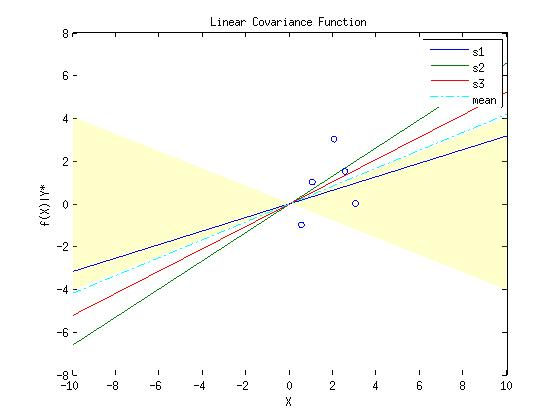
\includegraphics[width=0.8\textwidth]{1_e_1.jpg}
\caption{Linear Covariance Function}
\label{fig:1e1}
\end{figure}
\begin{figure}[H]
\centering
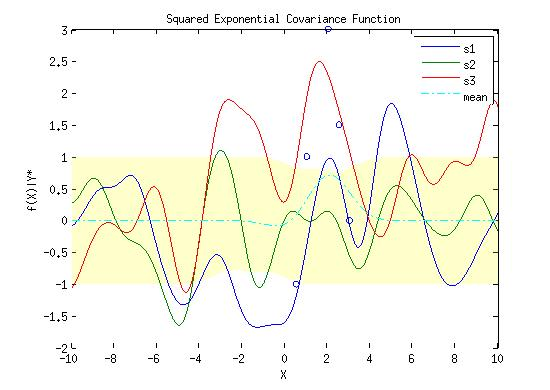
\includegraphics[width=0.8\textwidth]{1_e_2.jpg}
\caption{Square Exponential Covariance Function}
\label{fig:1e2}
\end{figure}
\begin{figure}[H]
\centering
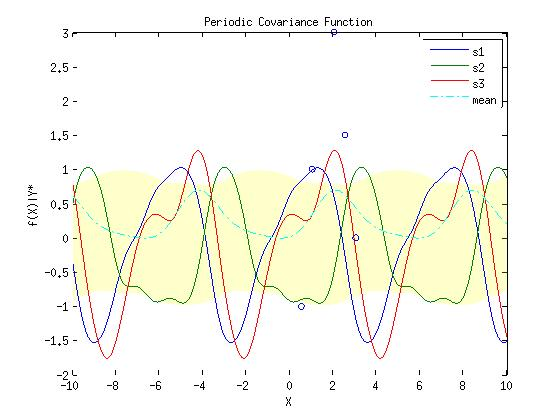
\includegraphics[width=0.8\textwidth]{1_e_3.jpg}
\caption{Periodic Covariance Function}
\label{fig:1e3}
\end{figure}

\item Figures~\ref{fig:1f1},~\ref{fig:1f2}, and~\ref{fig:1f3} show $f(X)|Y_\ast$ plotted for increasing values of $\lambda^2$.
%$\lambda^2$ seems to work as a smoothing factor -- the function gets smoother as $\lambda^2$ increases.
Smaller values of $\lambda^2$ result in higher variance and lower bias, whereas larger values
of $\lambda^2$ result in lower variance and higher bias. The function is more unstable for smaller values
of $\lambda^2$, (i.e., changing the training points would significantly change the function), 
than for large values of $\lambda^2$.


\begin{figure}[H]
\centering
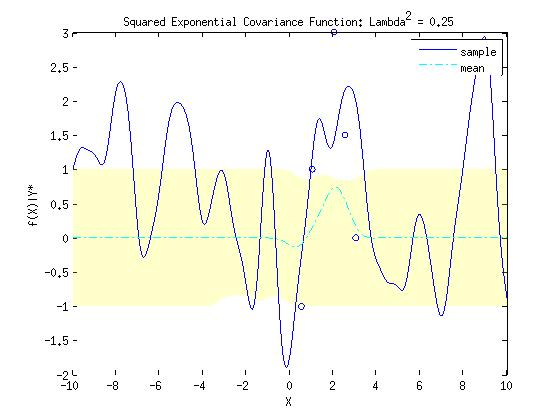
\includegraphics[width=0.8\textwidth]{1_f_1.jpg}
\caption{Sampling Different $\lambda^2$ Parameters Using the Squared Exponential Function}
\label{fig:1f1}
\end{figure}

\begin{figure}[H]
\centering
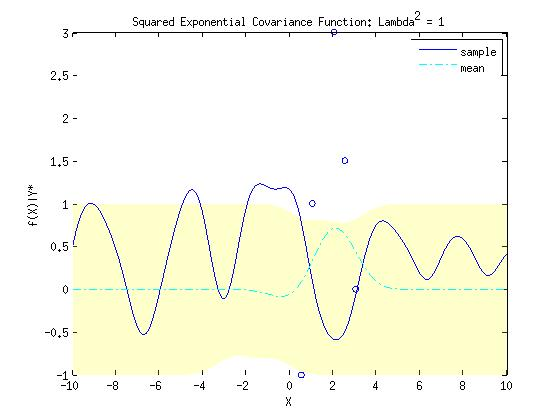
\includegraphics[width=0.8\textwidth]{1_f_2.jpg}
\caption{Sampling Different $\lambda^2$ Parameters Using the Squared Exponential Function}
\label{fig:1f2}
\end{figure}

\begin{figure}[H]
\centering
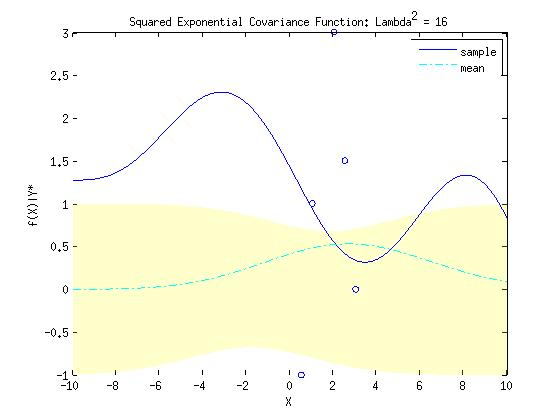
\includegraphics[width=0.8\textwidth]{1_f_3.jpg}
\caption{Sampling Different $\lambda^2$ Parameters Using the Squared Exponential Function}
\label{fig:1f3}
\end{figure}

\end{enumerate}
\end{document}